A continuación se presentan y discuten los resultados obtenidos tras ejecutar la batería experimental para el ordenamiento de arreglos y la multiplicación matricial. Se seleccionaron las configuraciones más representativas para contrastar empíricamente el comportamiento asintótico con la realidad del hardware.

\subsection{Ordenamiento de Arreglos Unidimensionales}

Para el problema de ordenamiento se evaluaron los cuatro algoritmos sobre arreglos de tamaño $N \in \{10^1, 10^3, 10^5, 10^7\}$ bajo diversas ordenaciones y dominios numéricos. En la Figura~\ref{fig:sorting_aleatorio} y Figura~\ref{fig:sorting_ascendente} se ilustran los desempeños para entradas aleatorias y ordenadas ascendentemente.

\begin{figure}[htbp]
    \centering
    \begin{minipage}{0.48\textwidth}
        \centering
        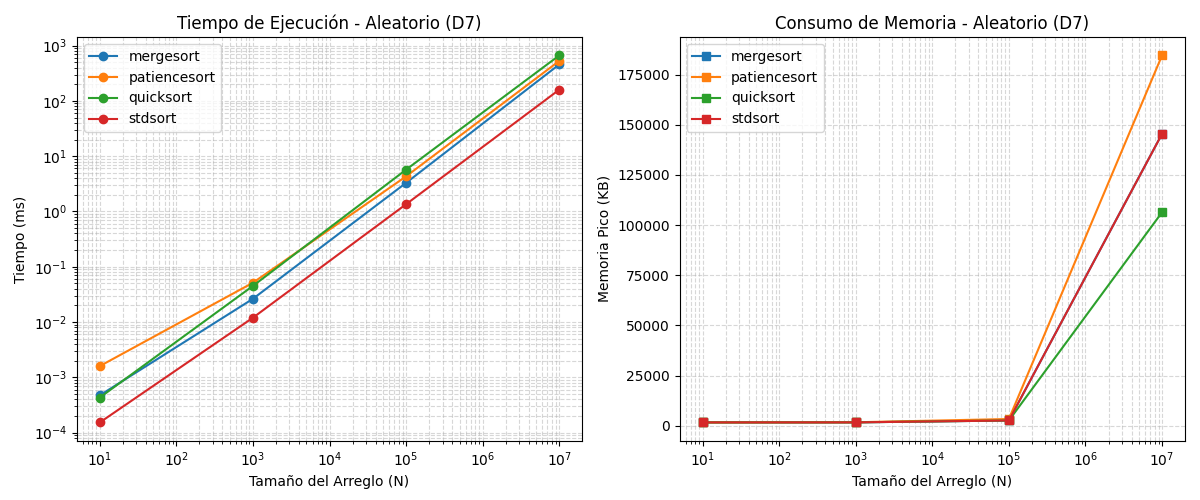
\includegraphics[width=\linewidth]{plots/sorting_aleatorio_D7.png}
        \caption{Tiempo y memoria en arreglos aleatorios ($D7$).}
        \label{fig:sorting_aleatorio}
    \end{minipage}\hfill
    \begin{minipage}{0.48\textwidth}
        \centering
        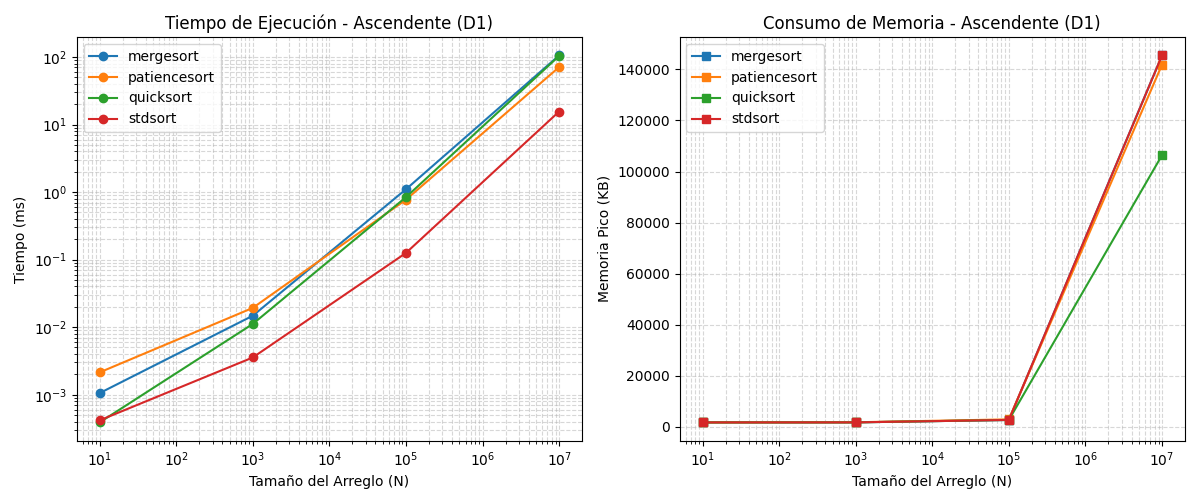
\includegraphics[width=\linewidth]{plots/sorting_ascendente_D1.png}
        \caption{Tiempo y memoria en arreglos ordenados ($D1$).}
        \label{fig:sorting_ascendente}
    \end{minipage}
\end{figure}

\begin{table}[htbp]
\centering
\small
\caption{Tiempo de ejecución promedio (ms) y memoria pico (KB) para $N = 10^7$.}
\label{tab:sorting_summary}
\begin{tabular}{llrrrr}
\toprule
\textbf{Distribución} & \textbf{Métrica} & \textbf{MergeSort} & \textbf{QuickSort} & \textbf{PatienceSort} & \textbf{std::sort} \\
\midrule
Aleatorio ($D7$) & Tiempo (ms)  & 456.57  & 665.17  & 528.96  & 159.60 \\
                 & Memoria (KB) & 145499  & 106405  & 184603  & 145483 \\
\midrule
Ascendente ($D1$) & Tiempo (ms)  & 105.40  & 103.70  & 70.80   & 15.57  \\
                  & Memoria (KB) & 145493  & 106405  & 141877  & 145488 \\
\bottomrule
\end{tabular}
\end{table}

\paragraph{Análisis de Tiempo de Ejecución:}
En las gráficas en escala logarítmica doble se observa que los cuatro algoritmos exhiben pendientes cuasi-lineales consistentes con su cota teórica de caso promedio $\Theta(N \log N)$.
\begin{itemize}
    \item \textbf{std::sort (Introsort):} Domina consistentemente con la menor constante oculta. Al combinar QuickSort con InsertionSort para particiones pequeñas y evitar recursión excesiva, minimiza los fallos de caché L1/L2 a nivel de arquitectura.
    \item \textbf{QuickSort y la Partición de Hoare:} La implementación con selección de pivote aleatorio y partición bidireccional de Hoare neutralizó el peor caso cuadrático $\Theta(N^2)$ reportado en particiones de Lomuto ante datos repetidos (dominio $D1$). Como se aprecia en la Figura~\ref{fig:sorting_ascendente}, para $N=10^7$ en $D1$, QuickSort culmina en $\approx 103.70$ ms, manteniendo la tasa $\mathcal{O}(N \log N)$.
    \item \textbf{PatienceSort:} Presenta un excelente rendimiento temporal en arreglos casi ordenados, pero sufre una sobrecarga en dominios amplios y aleatorios debido al costo logarítmico dinámico de balancear las pilas en la cola de prioridad (\texttt{std::priority\_queue}).
\end{itemize}

\paragraph{Análisis de Consumo de Memoria:}
Para $N \le 10^5$, el consumo de memoria se mantiene plano ($\approx 1800$ KB) dominado por el espacio base del proceso del sistema operativo. Sin embargo, en $N = 10^7$ se aprecian las diferencias estructurales:
\begin{itemize}
    \item \textbf{QuickSort} es el más eficiente ($\approx 106$ MB) debido a que opera \textit{in-place}, requiriendo únicamente espacio auxiliar $\mathcal{O}(\log N)$ en la pila de llamadas del procesador.
    \item \textbf{MergeSort} y \textbf{std::sort} demandan $\approx 145$ MB, producto del arreglo auxiliar indispensable para la fase de intercalación (\textit{merge}) de costo $\Theta(N)$.
    \item \textbf{PatienceSort} alcanza hasta $\approx 185$ MB en arreglos aleatorios y hasta $\approx 500$ MB en el peor caso de secuencias estrictamente decrecientes, debido al coste de punteros y nodos asociados a múltiples estructuras dinámicas (\texttt{std::vector<std::vector<int>>}).
\end{itemize}

\subsection{Multiplicación de Matrices Cuadradas}

Para la multiplicación de matrices se evaluaron instancias cuadradas de dimensión $N \in [2^1, 2^8]$ ($2 \le N \le 256$). En la Figura~\ref{fig:matrix_densa} y Figura~\ref{fig:matrix_dispersa} se contrastan las métricas temporales y espaciales para matrices densas y dispersas.

\begin{figure}[htbp]
    \centering
    \begin{minipage}{0.48\textwidth}
        \centering
        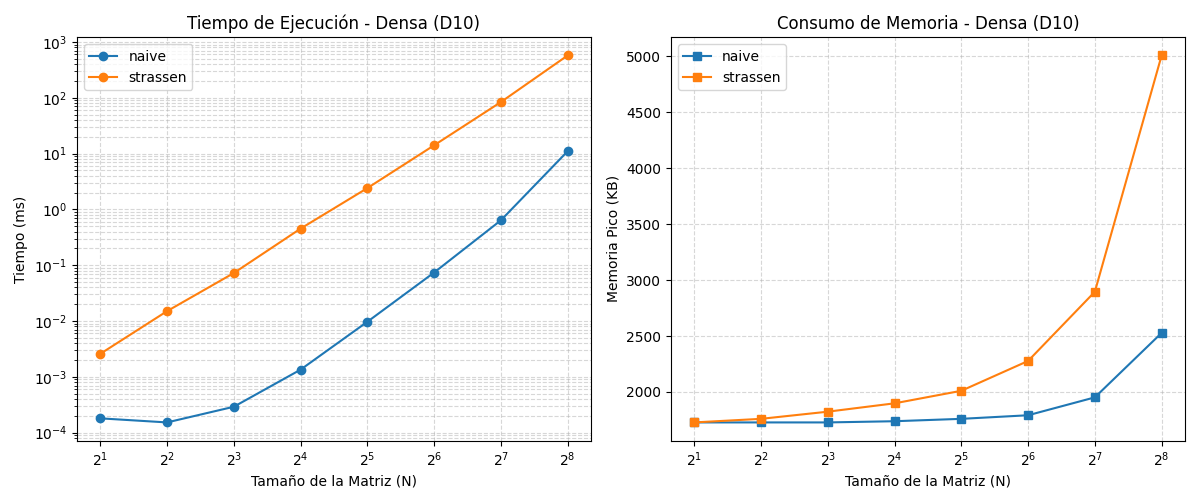
\includegraphics[width=\linewidth]{plots/matrix_densa_D10.png}
        \caption{Rendimiento en matrices densas ($D10$).}
        \label{fig:matrix_densa}
    \end{minipage}\hfill
    \begin{minipage}{0.48\textwidth}
        \centering
        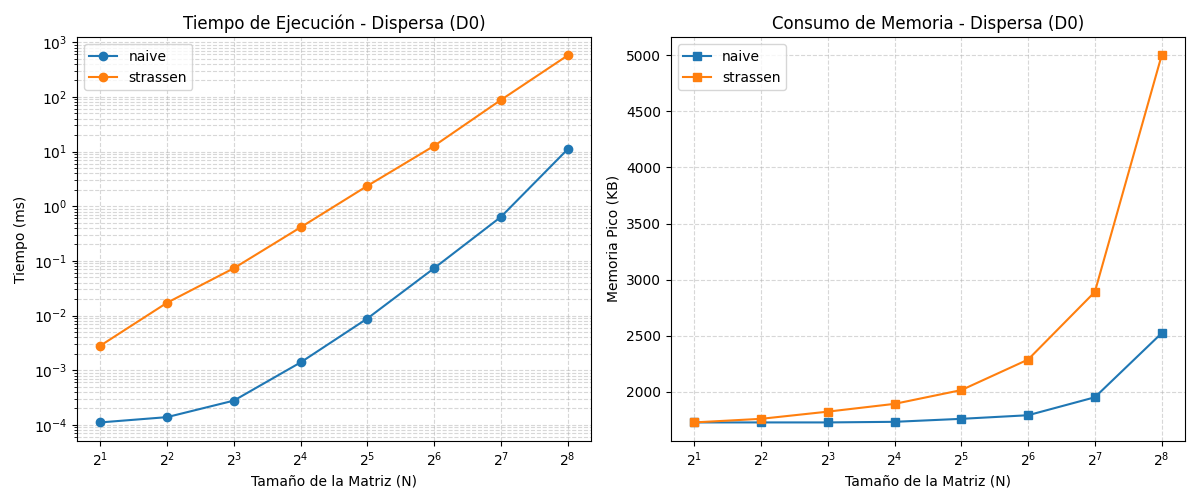
\includegraphics[width=\linewidth]{plots/matrix_dispersa_D0.png}
        \caption{Rendimiento en matrices dispersas ($D0$).}
        \label{fig:matrix_dispersa}
    \end{minipage}
\end{figure}

\begin{table}[htbp]
\centering
\small
\caption{Tiempo (ms) y memoria pico (KB) en multiplicación de matrices densas ($D10$).}
\label{tab:matrix_summary}
\begin{tabular}{rrrrr}
\toprule
& \multicolumn{2}{c}{\textbf{Tiempo de CPU (ms)}} & \multicolumn{2}{c}{\textbf{Memoria RAM Pico (KB)}} \\

\textbf{Dimensión ($N$)} & \textbf{Naive} & \textbf{Strassen} & \textbf{Naive} & \textbf{Strassen} \\
\midrule
$2^1 = 2$    & 0.0002 & 0.0026 & 1728 & 1728 \\
$2^4 = 16$   & 0.0013 & 0.4532 & 1739 & 1899 \\
$2^6 = 64$   & 0.0741 & 14.114 & 1792 & 2277 \\
$2^7 = 128$  & 0.6390 & 84.039 & 1952 & 2896 \\
$2^8 = 256$  & 11.064 & 575.37 & 2528 & 5008 \\
\bottomrule
\end{tabular}
\end{table}

\paragraph{Análisis de Desempeño y Sobrecarga Práctica:}
A pesar de que el Teorema Maestro establece para Strassen una cota asintótica estrictamente superior de $\mathcal{O}(N^{\log_2 7}) \approx \mathcal{O}(N^{2.81})$ frente a $\Theta(N^3)$ del método iterativo tradicional, los resultados experimentales demuestran que \textbf{el algoritmo Naive supera categóricamente a Strassen en todo el rango evaluado ($N \le 256$)}.

Esta aparente contradicción entre teoría y práctica se justifica mediante tres fenómenos del modelo computacional real:
\begin{enumerate}
    \item \textbf{Constante Oculta Desproporcionada:} En cada nivel del árbol de recursión, Strassen efectúa 18 sumas y restas de bloques de matrices de tamaño $(N/2) \times (N/2)$, además de alocar dinámicamente espacio para 21 matrices intermedias ($a, \dots, h$, $p_1, \dots, p_7$, auxiliares). La constante multiplicativa oculta en el término $\Theta(N^2)$ de la recurrencia $T(N) = 7T(N/2) + \Theta(N^2)$ es órdenes de magnitud mayor que la del bucle triple de Naive.
    \item \textbf{Dispersión de Memoria y Líneas de Caché:} Los tres bucles anidados de Naive acceden a posiciones secuenciales de memoria, aprovechando de forma óptima el principio de localidad espacial de las líneas de caché L1/L2. Strassen, al fragmentar los arreglos en matrices no contiguas en el \textit{heap}, multiplica los fallos de caché de datos (\textit{cache misses}).
    \item \textbf{Ausencia de Caso Base Híbrido:} El algoritmo de Strassen evaluado recurre de forma pura hasta submatrices de $1 \times 1$. En la literatura especializada se demuestra que para que Strassen sea competitivo, debe conmutar a multiplicación Naive cuando $N \le 64$ o $N \le 128$, y su punto de cruce real sobrepasa típicamente $N = 1024$ o $N = 2048$.
\end{enumerate}

\paragraph{Invarianza frente a la Dispersión:}
Se observa que las curvas para matrices densas, diagonales y dispersas son indistinguibles entre sí. Esto se debe a que ninguno de los dos algoritmos posee bifurcaciones condicionales que detecten coeficientes nulos; ambos aplican ciegamente la misma cantidad fija de operaciones aritméticas en el modelo \textit{word-RAM}.

\paragraph{Consumo de Memoria Residente:}
Tal como ilustra la Figura~\ref{fig:matrix_densa}, el consumo de memoria de Naive crece a una tasa cuadrática moderada asociada únicamente a las entradas $M_1, M_2$ y la salida $C$ ($\approx 2.5$ MB en $N=256$). Por su parte, Strassen escala de forma abrupta a partir de $N = 128$, alcanzando $\approx 5$ MB en $N=256$, producto de los múltiples marcos de pila y la retención de las matrices temporales $P_i$ en los diferentes niveles de la recursión.